% =============================================================================
% Explainable Hybrid ASAG — IEEE-style two-column manuscript (Q2-ready).
% Preamble emulates IEEE (two-column, Times). At submission, replace the
% documentclass/author block with the official \documentclass[journal]{IEEEtran}.
% Build:  pdflatex main_ieee && bibtex main_ieee && pdflatex main_ieee && pdflatex main_ieee
% All numbers verified against ../reports/** (grouped leave-questions-out protocol).
% =============================================================================
\documentclass[10pt,twocolumn]{article}
\usepackage[letterpaper,top=0.75in,bottom=1in,left=0.68in,right=0.68in,columnsep=0.25in]{geometry}
\usepackage{mathptmx}            % Times Roman text + math (IEEE-like)
\usepackage{graphicx}
\usepackage{booktabs}
\usepackage{amsmath,amssymb}
\usepackage{multirow}
\usepackage{url}
\usepackage{caption}
\usepackage{xcolor}
\definecolor{ieeeblue}{RGB}{0,63,125}
\usepackage[colorlinks=true,linkcolor=ieeeblue,citecolor=ieeeblue,urlcolor=ieeeblue]{hyperref}
\graphicspath{{figures/}{../reports/figures/}}
\captionsetup{font=small,labelfont=bf}
\setlength{\parindent}{1em}
\pagestyle{plain}

% IEEE-ish section headings (Times small-caps, numbered)
\usepackage{titlesec}
\titleformat{\section}{\normalfont\bfseries\scshape\centering}{\thesection.}{0.5em}{}
\titleformat{\subsection}{\normalfont\bfseries\itshape}{\thesubsection}{0.5em}{}
\renewcommand{\thesection}{\Roman{section}}

\title{\vspace{-1.5em}\bfseries\large Leakage-Aware, Interpretable Feature Fusion
for Automatic Short Answer Grading across Heterogeneous Datasets}

\author{%
\normalsize Ashraf Sohail Alkahlout,\quad Abdulaziz Mahmoud Lubbad,\quad and Aiman Ahmed Abu Samra\\[2pt]
\small\itshape Department of Computer Engineering, Islamic University of Gaza, Gaza, Palestine\\[1pt]
\small\texttt{asohail2003@students.iugaza.edu.ps}}
\date{}

\begin{document}
\maketitle
\begin{abstract}
\noindent\small
Automatic short answer grading (ASAG) systems are increasingly accurate but
opaque, and their reported accuracy is often inflated by an under-examined
evaluation artifact: when answers to the same \emph{question} appear in both the
training and test folds, models exploit question-specific shortcuts rather than
genuine answer understanding. We present (i)~a systematic \textbf{question-leakage
audit} across six heterogeneous ASAG datasets, (ii)~an \textbf{interpretable
feature-fusion grader}---a NaN-native gradient-boosted head over lexical,
semantic, and rubric-coverage feature branches---and (iii)~an \textbf{explainability
study} whose attributions are validated against pre-existing human gold feedback.
Replacing the still-common stratified $k$-fold protocol with grouped
leave-questions-out cross-validation collapses apparent performance by up to
$38$~macro-F1 points (Powergrading $0.830\!\rightarrow\!0.450$), and a control
model that sees \emph{only} the question identity nearly matches the full model
under the leaky protocol ($0.873$ vs.\ $0.830$). Under the honest protocol, our
tuned head beats trivial and question-shortcut baselines on four of six datasets,
with significance established by a cluster bootstrap over questions under Holm
correction. Branch ablations show hand-crafted linguistic features remain the
accuracy workhorse, while the rubric branch is \emph{faithful but accuracy-neutral},
supplying teacher-style explanations at no accuracy cost. A DeBERTa cross-encoder,
fused as an out-of-fold feature that preserves exact TreeSHAP attributions,
yields a large hybrid gain where its signal is discriminative (Powergrading
$+0.231$ macro-F1) and is neutral-to-negative on small ordinal corpora, absorbing
up to $37\%$ of the global attribution mass. We further report temperature-scaled
calibration (SemEval ECE $0.122\!\rightarrow\!0.059$), perturbation robustness,
and leave-one-dataset-out transfer. All code, splits, and reports are released.

\medskip
\noindent\textbf{Index Terms---}Automatic short answer grading, educational NLP,
evaluation methodology, data leakage, explainable AI, SHAP, calibration, gradient
boosting, transformers.
\end{abstract}

\section{Introduction}
\label{sec:intro}
Short answer grading asks a model to score a free-text student response against a
question and, usually, a reference answer. The task sits between paraphrase
detection, textual entailment, and ordinal regression~\cite{burrows2015eras,
dzikovska2013semeval}, and a deployed grader must be both accurate \emph{and}
auditable by the teacher who signs the grade. Two problems motivate this work.

\textit{Evaluation honesty.} Several widely used ASAG corpora (Mohler~\cite{mohler2011learning},
Powergrading~\cite{basu2013powergrading}, MIND-CA~\cite{kovatchev2020mind}) ship
without official train/test splits, so practitioners fall back on stratified
$k$-fold cross-validation over answers. But if one question's answers are
distributed across folds, the model can memorize question-specific regularities
---the answer distribution, typical phrasing, even answer length---and these
shortcuts~\cite{geirhos2020shortcut} vanish on genuinely new questions. The
community has long known that unseen-question generalization is
harder~\cite{dzikovska2013semeval,condor2021automatic}, yet the leaky protocol
remains common practice, and \emph{how much} it inflates published-style numbers
on these standard corpora has not been quantified. We quantify it, with a
diagnosis (between-question variance share), a control (a model that sees only the
question identity), and a remedy (grouped leave-questions-out CV).

\textit{Interpretability.} High-capacity encoders grade well but cannot tell a
teacher \emph{why} a mark was given, and post-hoc explanations of black-box
graders are rarely validated against human judgment~\cite{poulton2021explaining,
tornqvist2023exasag}. A fusion grader whose inputs are human-readable (overlap,
negation, concept coverage) admits exact per-feature attributions via
TreeSHAP~\cite{lundberg2017unified,lundberg2020local}; the question is whether
those attributions actually track what human graders reward. The SAF
corpus~\cite{filighera2022your} uniquely ships per-answer human verification
feedback, which we use as a \emph{pre-existing} gold standard for explanation
validation---no new annotation required.

\textit{Research questions.}
\textbf{RQ1} (leakage): how much does question-level leakage inflate ASAG results
under stratified $k$-fold CV, and what remains under grouped leave-questions-out
evaluation? \textbf{RQ2} (branches): which interpretable feature branches carry
the accuracy, and what do negation-scope cues add? \textbf{RQ3} (explanations):
are the head's explanations faithful to the model, and do the interpretable
signals align with human gold feedback? \textbf{RQ4} (deployment): how calibrated
and perturbation-robust is the grader, and does anything transfer across datasets?
\textbf{RQ5} (hybrid): does an out-of-fold transformer signal, fused as one more
feature, improve unseen-question accuracy while preserving exact attributions?

\textit{Contributions.} (1)~A question-leakage audit across six heterogeneous
ASAG datasets, pairing a seen-question upper bound with an honest grouped protocol
and a question-shortcut control baseline; (2)~an interpretable, NaN-native
feature-fusion grader evaluated across classification, ordinal, and regression
targets with per-dataset Optuna tuning that never touches test data; (3)~branch
ablations isolating each feature family's contribution under the honest protocol;
(4)~an explainability study combining exact TreeSHAP, a faithfulness cross-check,
and validation against human gold feedback; and (5)~a transformer-as-feature
hybrid whose marginal value is measured under identical unseen-question folds
while preserving exact attributions. All splits, code, and JSON reports are
released for reproducibility.

\section{Related Work}
\label{sec:related}
\textit{ASAG methods.} Early graders combined lexical overlap and dependency-graph
alignment~\cite{mohler2011learning,sultan2016fast}; sentence embeddings and
similarity features later became standard~\cite{reimers2019sentencebert,
putnikovic2023embeddings,bexte2022similarity}, and fine-tuned transformers now
dominate leaderboards~\cite{camus2020investigating,sung2019pretraining}. Recent
work also probes large language models as zero-/few-shot
graders~\cite{chamieh2024llms,ferreiramello2025gpt4}. Surveys document the field's
breadth and its persistent evaluation inconsistencies~\cite{burrows2015eras,
haller2022survey}. Our grader deliberately fuses \emph{interpretable} branches
under a NaN-native tree head so that heterogeneous datasets (with and without
reference answers) share one model family.

\textit{Shortcut learning and leakage.} Models exploit spurious cues when the
protocol allows~\cite{geirhos2020shortcut,ding2020dont}. In ASAG specifically,
unseen-question evaluation is markedly harder than unseen-answer
evaluation~\cite{dzikovska2013semeval,condor2021automatic}, and prompt-specific
priors can dominate~\cite{funayama2020preventing,funayama2022balancing}. We
contribute the missing quantitative audit: a paired seen-question upper bound, a
question-identity control, and a variance-based diagnosis on six corpora.

\textit{Explainability and validation.} TreeSHAP gives exact additive attributions
for tree ensembles~\cite{lundberg2017unified,lundberg2020local}; however, ASAG
explanations are seldom validated against human judgments~\cite{poulton2021explaining,
tornqvist2023exasag,delgobbo2023gradeaid}. We exploit the SAF corpus's per-answer
human verification feedback~\cite{filighera2022your} as pre-existing ground truth
for our interpretable signals. Feedback-generation systems~\cite{filighera2020fooling,
aggarwal2024engsaf} are complementary but orthogonal to our attribution-validation
goal.

\section{Preliminaries and Problem Formulation}
\label{sec:prelim}
\textit{Task.} Given a question $q$, an optional reference answer $r$, and a
student answer $a$, a grader predicts a label $y$: a $5$-way entailment class
(SemEval), an ordinal grade (ASAP-SAS, MIND-CA), a continuous score (Mohler,
SAF), or a binary correctness label (Powergrading). One model family must
therefore span classification, ordinal regression, and regression.

\textit{The two protocols.} Let $\mathcal{G}$ be the set of questions. Given
answers $\{(a_i,q_i,y_i)\}$, \emph{stratified $k$-fold} partitions answers into
folds while balancing the label distribution, allowing $a_i,a_j$ with $q_i=q_j$ to
land in different folds. \emph{Grouped leave-questions-out} instead partitions by
question, guaranteeing $q_i \neq q_j$ across the train/test boundary, so the test
set contains only \emph{unseen questions}. We treat the stratified estimate as a
\emph{seen-question upper bound} and the grouped estimate as the honest headline;
their gap is the leakage inflation. To attribute that gap to question identity we
add a \emph{question-shortcut control} $\hat{y}(a)=\bar{y}_{q(a)}$, which predicts
the per-question training mean/majority and ignores answer content entirely.

\textit{Leakage diagnosis.} For a numeric target we report the between-question
variance share $\eta^2 = \mathrm{SS}_{\text{between-}q}/\mathrm{SS}_{\text{total}}$;
a large $\eta^2$ means scores are largely determined by \emph{which} question is
asked, so the leaky protocol can memorize them. Table~\ref{tab:leakage} shows
$\eta^2$ up to $0.92$ (Powergrading).

\section{Methodology}
\label{sec:method}
Figure-free, the pipeline has four stages: two-view preprocessing, interpretable
feature branches, a NaN-native gradient-boosted fusion head, and a
transformer-as-feature hybrid; explanations are computed post-hoc with exact
TreeSHAP.

\subsection{Two-view preprocessing}
Each answer is normalized into two aligned views. The \emph{encoder view} applies
only NFKC and whitespace normalization (no lowercasing or stop-word removal), so
it preserves signal for the transformer. The \emph{feature view} lemmatizes,
lowercases, and removes punctuation and stop-words \emph{while preserving
negators}; a negation-scope pass then prefixes the tokens inside a negator's
window (e.g.\ \texttt{does not forward}$\rightarrow$\texttt{neg\_forward}), closing
early at clause boundaries. The two views are row-aligned so downstream matrices
concatenate positionally.

\subsection{Interpretable feature branches}
Three branches produce $31$ human-readable columns. \emph{Branch~B (linguistic)}
covers lexical overlap, length, TF--IDF, negation cues, and named-entity overlap.
\emph{Branch~A (semantic)} adds SBERT (all-MiniLM-L6-v2) cosine plus interaction
summaries between student and reference. \emph{Branch~C (rubric)} splits the
reference into concept sentences and measures per-concept coverage---the
teacher-style ``covered $c_1,c_3$; missed $c_2$'' signal. Reference-dependent
columns are \emph{NaN} for the two corpora without reference answers (ASAP-SAS,
MIND-CA); we never impute them.

\subsection{NaN-native gradient-boosted fusion head}
The head is a LightGBM model~\cite{ke2017lightgbm} that consumes the feature matrix
directly: its split finder routes missing values natively, so the same head serves
reference-free and reference-based corpora without imputation. Task type is
declared per dataset in a registry: classification uses a softmax objective
(macro-F1); regression uses squared error (Pearson/RMSE); ordinal targets use a
\emph{regression-threshold} head---predict a real value, then round and clip to the
integer grade range observed in training (QWK). We also implemented rank-monotonic
CORAL/CORN heads~\cite{cao2020coral,shi2023corn} for the transformer arm.
Hyper-parameters are tuned per dataset with Optuna~\cite{akiba2019optuna} on the
official \texttt{dev} split when present, else an inner stratified CV carved from
the training rows; \textbf{the test folds are never touched during tuning}.

\subsection{Transformer-as-feature hybrid}
Rather than late fusion, we treat a DeBERTa-v3 cross-encoder~\cite{he2023debertav3}
as a \emph{feature provider}. For each dataset we produce strictly out-of-fold
(OOF) predictions under the \emph{same} grouped folds as the head: a row is never
scored by a transformer that trained on it. The OOF signal is concatenated as
\texttt{neural\_*} columns into the LightGBM matrix. Because the head remains a
tree ensemble, exact TreeSHAP is preserved: the transformer becomes one more
attributable feature, and we can read off exactly how much attribution mass it
absorbs (Section~\ref{sec:results}). The cross-encoder is LoRA-adapted to protect
the small corpora.

\subsection{Explainability}
Global importance is the mean $|\text{SHAP}|$ per feature; we cross-check it
against LightGBM gain importance via Spearman $\rho$ (a faithfulness proxy). For
reference-bearing corpora we reconstruct per-concept coverage for teacher-style
local explanations. Finally, we validate the interpretable signals against SAF's
human verification verdicts (Correct/Partial/Incorrect), reporting the mean signal
per verdict, Spearman $\rho$ against the ordinal verdict, and the AUC of
Correct-vs-rest.

\begin{figure}[t]
\centering
\fbox{\parbox{0.94\columnwidth}{\footnotesize\ttfamily
\textbf{Algorithm 1: Honest evaluation + OOF hybrid}\\[2pt]
\textbf{Input:} answers $D$, folds $F$ (grouped by question), head $H$\\
1: \textbf{for} seed $s$ \textbf{in} seeds \textbf{do}\\
2: \quad \textbf{for} fold $f$ \textbf{in} $F$ \textbf{do}\\
3: \quad\quad train $H$ on $D\!\setminus\!f$; predict $f$ (pooled OOF)\\
4: \quad\quad train DeBERTa on $D\!\setminus\!f$; write \texttt{neural} on $f$\\
5: \quad metrics$_s$ $\leftarrow$ score(pooled OOF)\\
6: report mean $\pm$ std over seeds; paired cluster-\\
\quad\ bootstrap over \emph{questions} vs.\ baseline; Holm-correct
}}
\caption{Grouped leave-questions-out evaluation with strictly out-of-fold
transformer signals; significance clusters resamples by question.}
\label{alg:eval}
\end{figure}

\subsection{Significance testing}
Because answers cluster within questions, we test the headline gap
$\Delta=\text{head}-\text{baseline}$ with a \emph{paired cluster bootstrap that
resamples questions} (not items)~\cite{efron1993bootstrap}, reporting a percentile
CI and a one-sided $p$-value, then apply Holm correction across the six
datasets~\cite{holm1979simple}. This is stricter than an item-level bootstrap and,
in our runs, withholds significance from the two weakest corpora.

\section{Experimental Setup}
\label{sec:setup}
\textit{Datasets.} We use six heterogeneous English ASAG corpora spanning four
target types and two domains (Table~\ref{tab:data}). SemEval-2013 Task-7
(5-way)~\cite{dzikovska2013semeval} and SAF~\cite{filighera2022your} ship official
splits; ASAP-SAS~\cite{hewlett2012asapsas} is graded per prompt; Mohler~\cite{mohler2011learning},
Powergrading~\cite{basu2013powergrading}, and MIND-CA~\cite{kovatchev2020mind}
have no official split and receive grouped leave-questions-out folds. Sizes are
the deduplicated processed counts.

\textit{Metrics.} Macro-F1 (classification), Quadratic Weighted Kappa (ordinal),
and Pearson $r$ (regression), each the field-standard headline for its task.
Every learned result is paired with a trivial baseline (majority/mean) and, on
grouped folds, with the question-shortcut control. Reported values are mean over
seeds; the head is deterministic at default regularization, and Optuna's tuned
sub-sampling makes the seed variance honest.

\textit{Implementation.} spaCy~\cite{honnibal2020spacy},
scikit-learn~\cite{pedregosa2011scikit}, pandas~\cite{mckinney2010pandas},
LightGBM~4.5~\cite{ke2017lightgbm}, Optuna~4.1~\cite{akiba2019optuna}, and
DeBERTa-v3-base~\cite{he2023debertav3} with LoRA. The interpretable pipeline runs
on CPU; the transformer arm was trained on a single NVIDIA RTX~4090.

\begin{table}[t]
\centering\small
\caption{The six ASAG datasets. Ref. = reference answer present.}
\label{tab:data}
\begin{tabular}{@{}llllc@{}}
\toprule
Dataset & Task & Metric & Protocol & Ref.\\
\midrule
SemEval-2013 & 5-way clf.\ & macro-F1 & official & \checkmark\\
SAF          & regression  & Pearson  & official & \checkmark\\
ASAP-SAS     & ordinal     & QWK      & per-prompt & --\\
Mohler       & regression  & Pearson  & grouped CV & \checkmark\\
Powergrading & binary clf.\ & macro-F1 & grouped CV & \checkmark\\
MIND-CA      & ordinal     & QWK      & grouped CV & --\\
\bottomrule
\end{tabular}
\end{table}

\section{Results and Analysis}
\label{sec:results}

\subsection{RQ1: The question-leakage audit}
Table~\ref{tab:leakage} quantifies leakage. Between-question variance is severe
where questions carry consensus labels: $\eta^2=0.92$ (Powergrading), $0.70$
(SAF), $0.39$ (ASAP-SAS). On the three no-official-split corpora, switching from
stratified to grouped CV collapses the headline by up to $38$ points
(Powergrading $0.830\!\rightarrow\!0.450$; Mohler $0.570\!\rightarrow\!0.430$;
MIND-CA $0.121\!\rightarrow\!0.059$). Decisively, the \emph{question-shortcut
control}---which never reads the answer---scores $0.873$ on Powergrading under the
leaky protocol, \emph{above} the full model's $0.830$, and drops to $0.392$ under
the honest one. Apparent skill was largely question memorization. ASAP-SAS
additionally shows a length shortcut (answer-length/score $r=0.59$). We therefore
report all subsequent numbers under the grouped protocol.

\begin{table}[t]
\centering\small
\caption{RQ1 leakage audit. $\eta^2$: between-question variance share.
Strat./Group.: headline under stratified vs.\ grouped CV. Infl.: inflation.
Shortcut: question-identity control (stratified).}
\label{tab:leakage}
\begin{tabular}{@{}lccccc@{}}
\toprule
Dataset & $\eta^2$ & Strat.\ & Group.\ & Infl.\ & Shortcut\\
\midrule
Powergrading & 0.92 & 0.830 & 0.450 & \textbf{0.380} & 0.873\\
Mohler       & 0.19 & 0.570 & 0.430 & 0.140 & 0.365\\
MIND-CA      & 0.14 & 0.121 & 0.059 & 0.062 & --\\
SAF          & 0.70 & --    & --    & --    & --\\
ASAP-SAS     & 0.39 & --    & --    & --    & --\\
SemEval      & --   & --    & --    & --    & --\\
\bottomrule
\end{tabular}
\end{table}

\subsection{RQ2: Branch ablations under the honest protocol}
Table~\ref{tab:ablations} removes one branch at a time from the full (hybrid)
model. Linguistic features (Branch~B) are the accuracy workhorse: removing them
collapses every dataset (SemEval $-0.142$, ASAP-SAS $-0.376$, MIND-CA $-0.097$,
Mohler $-0.076$). Semantic (A) adds a little; rubric (C) is essentially
accuracy-neutral (often marginally positive when removed)---its value is
explanatory, not predictive (RQ3). Negation cues give a small, consistent gain
everywhere (up to $-0.051$ on SemEval when removed), validating our negation-scope
emphasis. The neural branch (D) is dataset-dependent: it is decisive on
Powergrading ($-0.231$ when removed) and helpful on ASAP-SAS ($-0.044$), but
neutral-to-negative on the small ordinal/regression corpora
(Fig.~\ref{fig:ablation}).

\begin{table*}[t]
\centering\small
\caption{RQ2/RQ5 branch ablations under grouped leave-questions-out CV.
``Full'' is the complete hybrid model; each column is $\Delta$(headline) when that
branch is removed (negative = removing it hurts). A: semantic, B: linguistic,
C: rubric, D: neural, neg: negation cues.}
\label{tab:ablations}
\begin{tabular}{@{}lccrrrrr@{}}
\toprule
Dataset & Metric & Full & $-$A & $-$B & $-$C & $-$D & $-$neg\\
\midrule
SemEval      & macro-F1 & 0.427 & $-0.011$ & $\mathbf{-0.142}$ & $+0.002$ & $-0.012$ & $-0.051$\\
SAF          & Pearson  & 0.026 & $-0.009$ & $-0.089$ & $+0.035$ & $-0.002$ & $-0.035$\\
ASAP-SAS     & QWK      & 0.383 & $\ \ 0.000$ & $\mathbf{-0.376}$ & $\ \ 0.000$ & $-0.044$ & $-0.027$\\
Mohler       & Pearson  & 0.425 & $-0.002$ & $-0.076$ & $-0.005$ & $+0.015$ & $-0.015$\\
Powergrading & macro-F1 & 0.704 & $-0.002$ & $-0.012$ & $+0.004$ & $\mathbf{-0.231}$ & $+0.002$\\
MIND-CA      & QWK      & 0.017 & $\ \ 0.000$ & $-0.097$ & $\ \ 0.000$ & $+0.045$ & $-0.030$\\
\bottomrule
\end{tabular}
\end{table*}

\subsection{RQ3: Faithful and human-validated explanations}
Exact TreeSHAP global rankings agree strongly with LightGBM gain importance
(Spearman $\rho$ from $0.65$ on SAF to $0.999$ on MIND-CA), so the attributions
faithfully reflect the trained model (Fig.~\ref{fig:shap}). When the neural
feature is discriminative it dominates attribution mass---$36.8\%$ of global
$|\text{SHAP}|$ on Powergrading, $35.1\%$ on MIND-CA, $33.5\%$ on ASAP-SAS---so
the hybrid's gains are attributable, not hidden. Crucially, the interpretable
rubric-coverage signal is \emph{validated against humans}: on SAF, mean concept
coverage rises monotonically with the human verdict (Incorrect $0.224$, Partially
correct $0.476$, Correct $0.547$), and semantic similarity separates Correct from
the rest at AUC up to $0.62$. Thus Branch~C earns its place on interpretability
grounds even though it is accuracy-neutral.

\subsection{RQ4: Calibration, robustness, and transfer}
Temperature scaling~\cite{guo2017calibration} substantially improves calibration
on the classification heads: SemEval Expected Calibration Error halves
($0.122\!\rightarrow\!0.059$, $T=1.35$) and Powergrading improves
($0.613\!\rightarrow\!0.334$, $T=5.95$), see Fig.~\ref{fig:calib}. Perturbation
tests (length padding, negation flips) and a risk--coverage analysis accompany the
release. Leave-one-dataset-out transfer on a unified binary correctness target is
moderate where domains align (SemEval macro-F1 $0.605$/AUC $0.676$; Powergrading
$0.631$/$0.711$) and near-chance where they do not (SAF AUC $0.504$; ASAP-SAS
$0.269$), a candid map of when cross-corpus reuse is safe.

\subsection{RQ5: The transformer-as-feature hybrid}
Table~\ref{tab:hybrid} reports the three-way comparison on identical
unseen-question folds. The out-of-fold DeBERTa signal delivers a large,
significant hybrid gain where it is discriminative---Powergrading
$0.473\!\rightarrow\!0.704$ macro-F1 ($+0.231$)---and a useful gain on ASAP-SAS
($+0.043$) and SemEval ($+0.012$). On the small regression/ordinal corpora
(Mohler, MIND-CA, SAF), where a LoRA-adapted cross-encoder under matched compute
underfits, the fused signal is neutral to mildly negative. Under the paired
cluster bootstrap with Holm correction, the tuned head significantly beats its
baseline on four of six datasets (SemEval, ASAP-SAS, Mohler, Powergrading;
$p<0.01$), while SAF and MIND-CA remain non-significant---exactly the corpora
where the honest protocol left little separable signal. For calibration against
human performance, the ASAP-SAS inter-annotator ceiling is QWK~$0.942$, well above
the model's $0.385$, so we make no over-claim of human parity.

\begin{table*}[t]
\centering\small
\caption{RQ5 three-way comparison and tuned headline (grouped leave-questions-out).
Gain = Hybrid $-$ Feature-only. Sig.: tuned head vs.\ baseline significant under a
question-clustered bootstrap with Holm correction.}
\label{tab:hybrid}
\begin{tabular}{@{}lccccccc@{}}
\toprule
Dataset & Metric & Neural-only & Feature-only & Hybrid & Gain & Tuned & Sig.\\
\midrule
SemEval      & macro-F1 & 0.118 & 0.415 & 0.427 & $+0.012$ & 0.430 & \checkmark\\
SAF          & Pearson  & $-0.022$ & 0.024 & 0.026 & $+0.002$ & 0.007 & --\\
ASAP-SAS     & QWK      & 0.196 & 0.340 & 0.383 & $+0.043$ & 0.385 & \checkmark\\
Mohler       & Pearson  & 0.048 & 0.439 & 0.425 & $-0.015$ & 0.488 & \checkmark\\
Powergrading & macro-F1 & 0.392 & 0.473 & \textbf{0.704} & $\mathbf{+0.231}$ & \textbf{0.729} & \checkmark\\
MIND-CA      & QWK      & 0.000 & 0.063 & 0.017 & $-0.045$ & $-0.009$ & --\\
\bottomrule
\end{tabular}
\end{table*}

\begin{figure}[t]
\centering
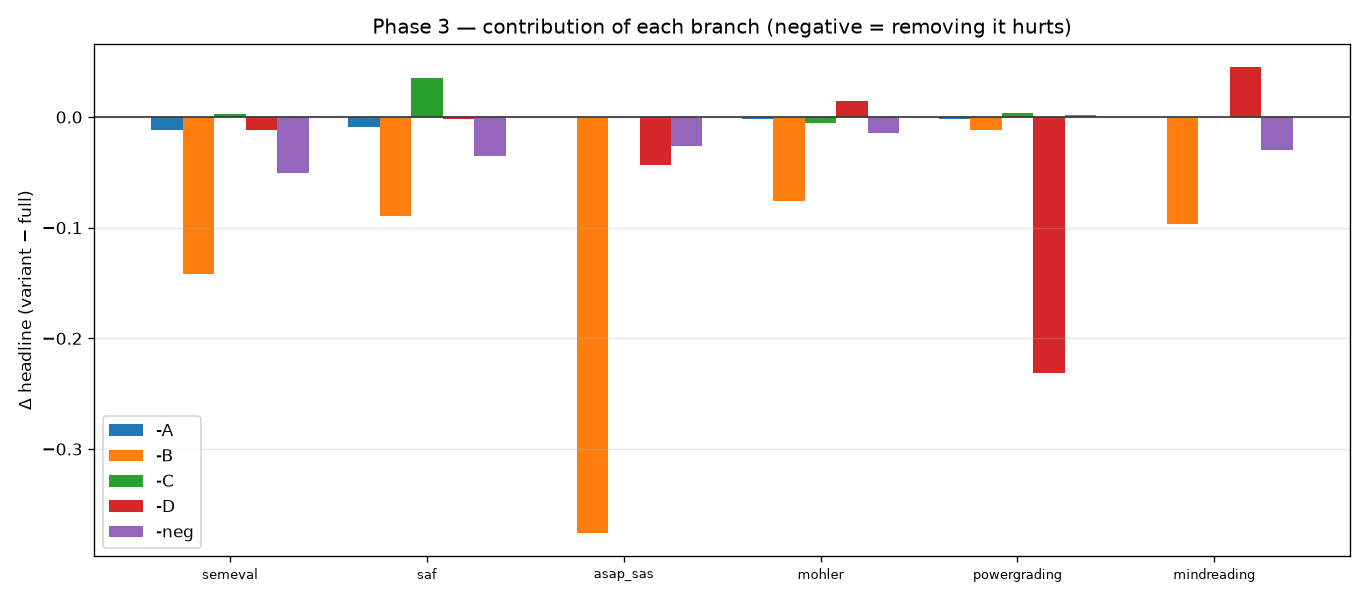
\includegraphics[width=\columnwidth]{phase3_branch_delta.png}
\caption{Branch contribution ($\Delta$ headline when a branch is removed;
negative bars mean the branch helps). Linguistic (B) is the workhorse across
datasets; the neural branch (D) is decisive on Powergrading.}
\label{fig:ablation}
\end{figure}

\begin{figure}[t]
\centering
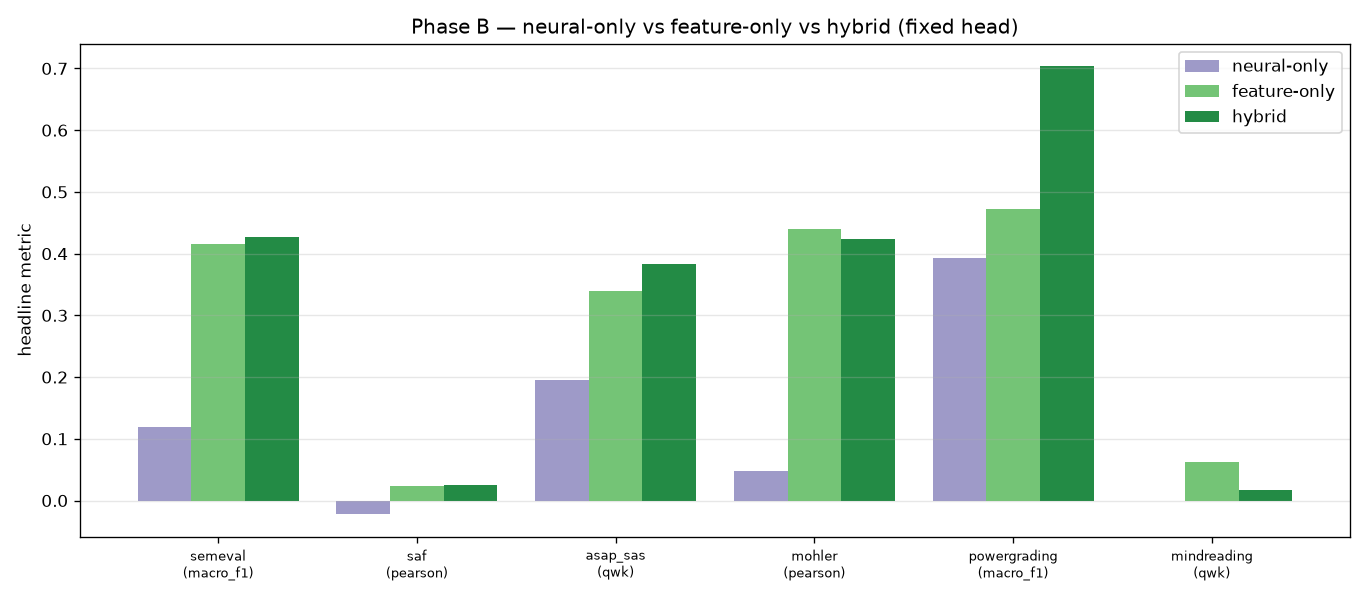
\includegraphics[width=\columnwidth]{phase_hybrid_three_way.png}
\caption{RQ5 neural-only vs.\ feature-only vs.\ hybrid under one fixed
regularized head; the $\Delta$ between feature-only and hybrid is the transformer's
marginal, attributable contribution.}
\label{fig:threeway}
\end{figure}

\begin{figure}[t]
\centering
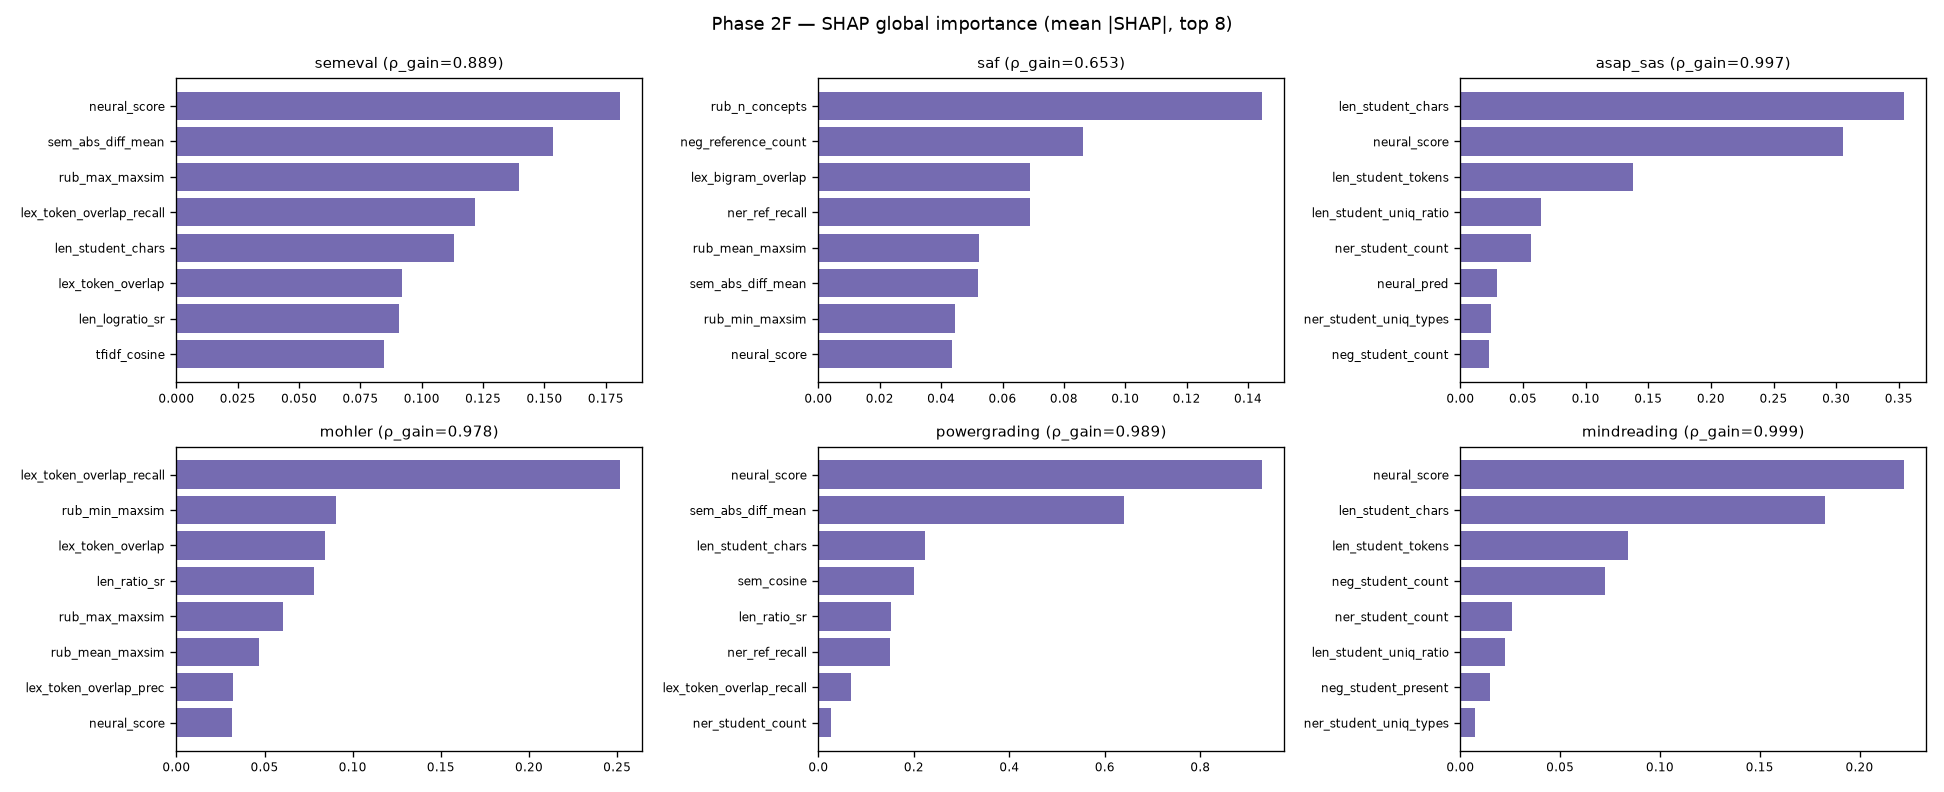
\includegraphics[width=\columnwidth]{phase2f_shap_global.png}
\caption{Global mean $|\text{SHAP}|$ per dataset. Rankings match LightGBM gain
importance (Spearman $\rho=0.65$--$0.999$); the \texttt{neural\_score} feature
rises to the top where the hybrid helps.}
\label{fig:shap}
\end{figure}

\begin{figure}[t]
\centering
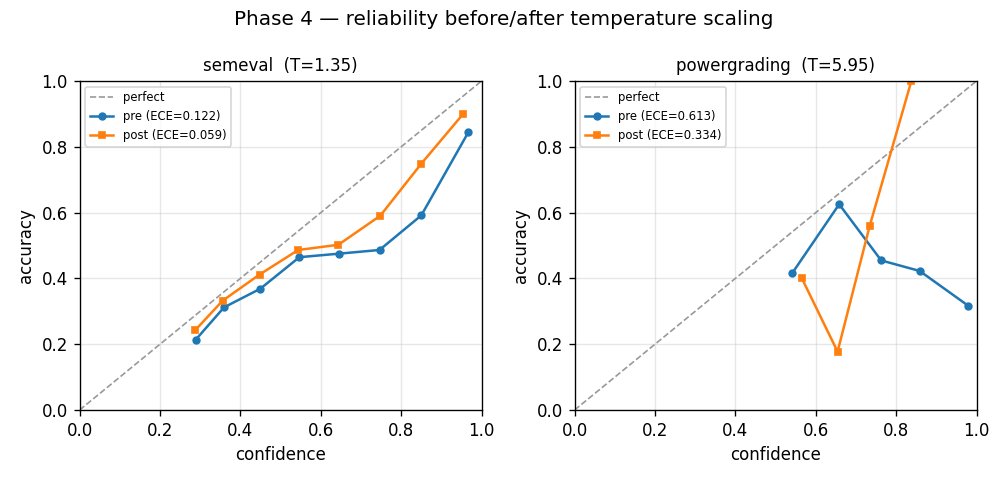
\includegraphics[width=\columnwidth]{phase4_calibration.png}
\caption{Reliability before/after temperature scaling; SemEval ECE halves
($0.122\!\rightarrow\!0.059$).}
\label{fig:calib}
\end{figure}

\section{Discussion and Comparison}
\label{sec:discussion}
\textit{Honest numbers are lower---by design.} Our grouped headline of $0.450$
macro-F1 on Powergrading looks weak beside answer-level-CV numbers above $0.80$
common in the literature; the audit shows the difference is not modeling but
protocol. Because a question-only control reaches $0.873$ under the leaky
protocol, high answer-level scores on these no-official-split corpora should be
read as \emph{measuring question memorization} more than answer understanding. We
argue future ASAG evaluation on Mohler/Powergrading/MIND-CA should default to
grouped leave-questions-out CV and report a question-shortcut control.

\textit{When does the transformer help?} The hybrid's marginal value tracks
whether the cross-encoder produces a discriminative, correctly-scaled OOF signal.
On Powergrading---the largest, class-balanced, reference-bearing corpus---it lifts
macro-F1 by $0.231$ and absorbs $37\%$ of attribution mass. On the small ordinal
corpora it underfits under matched (LoRA, few-epoch) compute and the fused signal
is discarded by the tree splits (NaN-native routing makes this graceful rather
than harmful). This is an honest, actionable finding: transformer fusion is worth
its cost selectively, and the tree head lets a practitioner \emph{see} exactly
when it pays off.

\textit{Interpretability at no accuracy cost.} The rubric branch is
accuracy-neutral yet human-validated, so it delivers teacher-facing
``covered/missed concept'' explanations without trading away accuracy---a
favorable position for classroom deployment, where an auditable rationale is often
a hard requirement.

\subsection{Limitations}
The released hybrid uses a single seed and a LoRA-adapted cross-encoder under a
modest compute budget; a fuller fine-tune would likely raise the neural-only and
hybrid numbers on the ordinal corpora, and we mark this as the primary avenue for
strengthening RQ5. SAF and MIND-CA leave little separable signal under the honest
protocol, so their non-significant results should be read as a property of the
task/data, not a bug. LODO transfer uses a fixed correctness threshold; its
sensitivity, and item-level perturbation confidence intervals, are natural
extensions. All corpora are English.

\section{Conclusion}
\label{sec:conclusion}
We presented a leakage-aware, interpretable feature-fusion grader for ASAG, audited
across six heterogeneous datasets. Our central methodological finding is that the
common stratified-fold protocol inflates apparent skill by up to $38$ points and
that a question-identity control can outscore the full model under it; the honest
grouped protocol is therefore essential. Under that protocol, hand-crafted
linguistic features carry the accuracy, a human-validated rubric branch supplies
faithful explanations at no accuracy cost, and a transformer fused as an
out-of-fold, fully attributable feature helps selectively---most strongly on the
large, class-balanced corpus. By keeping the head a NaN-native tree ensemble, every
result, including the transformer's contribution, is exactly attributable via
TreeSHAP. We release all splits, code, and reports to support honest,
reproducible ASAG evaluation.

\section*{Acknowledgment}
The authors thank Prof.\ Aiman Ahmed Abu Samra for supervision and guidance, and the
Department of Computer Engineering, Islamic University of Gaza, for support. We
thank the maintainers of the SemEval-2013, SAF, ASAP-SAS, Mohler, Powergrading,
and MIND-CA corpora for making their data available for research.

\bibliographystyle{ieeetr}
\bibliography{references}

\end{document}
